\subsection{Thai Word Segmentation Revisited}

In the early stage of Thai word segmentation, dictionary-based learning techniques had been used along with machine-learning techniques, for instance, Markov models \cite{Kawtrakul1997}, decision trees \cite{Sornlertlamvanich2000,Theeramunkong2001}, and CRFs \cite{Haruechaiyasak2008}.
%
CRFs have been shown to be particularly suitable for Thai sequence-labeling tasks \cite{Kruengkrai2006,Haruechaiyasak2009,Kruengkrai2009,Nararatwong2018}.
%

In parallel with CRFs, neural-network models, e.g., CNNs \cite{Kittinaradorn2019,Chormai2019}, LSTM \cite{Treeratpituk2017},\footnote{https://github.com/pucktada/cutkum} and BiLSTM \cite{Jousimo2017}, have been applied and performed excellently for character-based Thai word segmentation.
%
Using additional knowledge, such as CC \cite{Lapjaturapit2018,Nararatwong2018}, transfer learning \cite{seeha-etal-2020-thailmcut}, and stacking ensemble \cite{limkonchotiwat-etal-2020-domain,limkonchotiwat-etal-2021-handling}, along with neural-network models could improve performance.
%

\subsection{Character Clusters in Thai Word Segmentation}
Compared with English, the Thai language has various types of characters, i.e., consonants, vowels, tones, and special characters.
%
A word can be formed from a combination of these characters.
%
Thai also has unique linguistic phenomena, for example, some sequential characters tend to be indivisible units.
%
Thus, \citeA{Theeramunkong2000} introduced the concept of a CC, which is a set of predefined rules for an indivisible unit on the basis of the Thai writing system.
%

A CC is smaller than a word but larger than a character.
%
This concept is roughly comparable to a subword unit that is also in the middle of a character and word in terms of length. 
%
Using subword units, as well as CCs \cite{Theeramunkong2004,Sutantayawalee2015,Lapjaturapit2018,Nararatwong2018}, in word-segmentation tasks could yield good segmentation performance \cite{yang-etal-2019-subword,li-etal-2019-word-segmentation}.
%
However, decomposing subword units from words requires specific settings such as Byte Pair Encoding (BPE), while CCs do not require any additional settings.
%

A CC helps avoid segmenting that might violate a writing system \cite{Limcharoen2009}, while subword units will likely not thoroughly exploit morphology \cite{provilkov-etal-2020-bpe}, which could generate noise and weaken segmentation performance. 
%
This generally makes CCs smaller than subword units, as shown in Figure~\ref{fig:tccsub}, which enables a sample-comparison of segmentation results from coarse to fine (top-down) information.
%
\begin{figure}
    \centering
    \begin{subfigure}{0.49\textwidth}
        \centering
        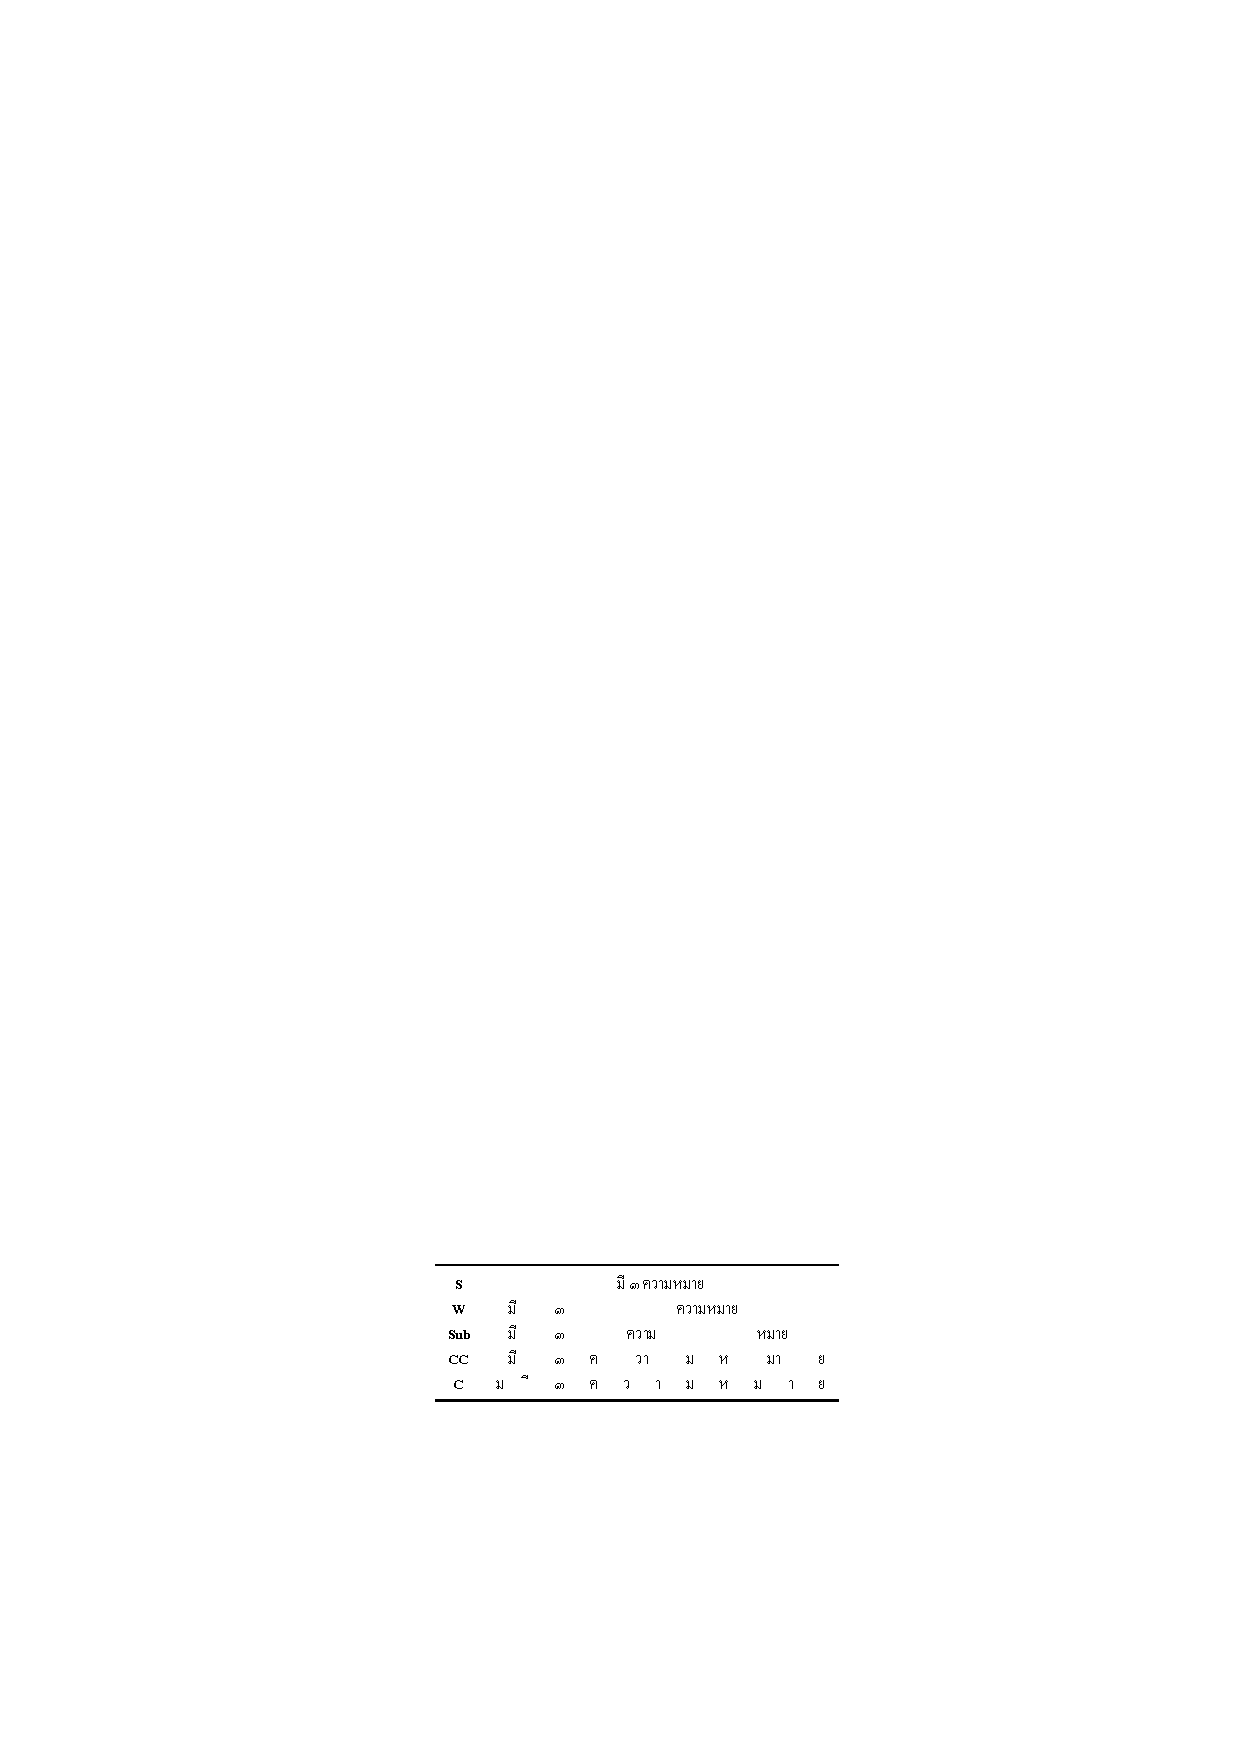
\includegraphics[width=\textwidth]{figures/fig-tccsub.pdf}
    \end{subfigure}
    \hspace{\textwidth}
    \begin{subfigure}{0.24\textwidth}
        \centering
        
\includegraphics[width=\textwidth]{figures/fig-thbies-tran.pdf}
    \end{subfigure}
    \caption{Comparison of segmentation results. S, W, Sub, CC, and C indicate segmentation levels of sentence, word, subword, character cluster, and character, respectively.}
    \label{fig:tccsub}
\end{figure}

\subsection{Pre-trained models in Thai Word Segmentation}
Recent research works show that pre-trained models are useful for many downstream tasks, particularly Chinese Word Segmentation (CWS) \cite{yang-etal-2019-bert,qiu-etal-2020-concise,ke-etal-2020-unified,huang-etal-2020-towards,ke-etal-2021-pre}.
%
\citeA{yang-etal-2019-bert} adopted a multi-layer Bidirectional Encoder Representation from Transformers (BERT) to subword-based CWS.
%
Comparing with several neural models i.e., CNNs and BiLSTM, their work could yield better segmentation performance.
%

To our best knowledge, only \citeA{seeha-etal-2020-thailmcut} that applies PTM to Thai word segmentation. 
%
They pre-trained character-based Language Model with BiLSTM architecture and then transferred its parameters for fine-tuning character-based word segmentation afterwards. 
%
This approach set state-of-the-art performance on BEST2010 dataset,\footnote{\url{https://thailang.nectec.or.th}} which is the most well-known Thai dataset for evaluating Thai word segmentation.

\subsection{Attention Mechanism}
An attention mechanism was initially proposed by \citeA{Bahdanau2015} for neural machine translation focusing on proper parts in sentences, particularly long sentences. 
%
Basically, the attention mechanism estimates attention vectors between source and target states.
%
It has been successfully applied to downstream tasks, including machine translation \cite{luong-etal-2015-effective,Vaswani2017}, constituency parsing \cite{kitaev-klein-2018-constituency}, and sequence-labeling \cite{higashiyama-etal-2019-incorporating,tian-etal-2020-joint-chinese}.
%